\documentclass[../main.tex]{subfiles}
\begin{document}

\section*{第1問}

% Source: handwritten.pdf 第1問．
{\bf [解]}
\begin{align}
  \overrightarrow{OP}&=(1-s)
  \begin{pmatrix}3\\0\\0
  \end{pmatrix}
  +s
  \begin{pmatrix}3\\0\\4
  \end{pmatrix}
  =
  \begin{pmatrix}3\\0\\0
  \end{pmatrix}+s
  \begin{pmatrix}0\\0\\4
  \end{pmatrix},\\
  \overrightarrow{OQ}&=(1-t)
  \begin{pmatrix}0\\2\\0
  \end{pmatrix}
  +t
  \begin{pmatrix}0\\2\\4
  \end{pmatrix}
  =
  \begin{pmatrix}0\\2\\0
  \end{pmatrix}+t
  \begin{pmatrix}0\\0\\4
  \end{pmatrix}.
\end{align}
だから，$AC$上の点$R$を
\begin{align}
  \overrightarrow{OR}=\alpha
  \begin{pmatrix}3\\0\\0
  \end{pmatrix}
  +(1-\alpha)
  \begin{pmatrix}0\\2\\0
  \end{pmatrix}
  =
  \begin{pmatrix}0\\2\\0
  \end{pmatrix}+\alpha
  \begin{pmatrix}3\\-2\\0
  \end{pmatrix}
  \quad(0\leqq\alpha\leqq1)
\end{align}
で定めて，$DR\perp OP$かつ$DR\perp OQ$なる$\alpha$の存在条件をもとめれば良い．
\begin{figure}[H]
  \begin{center}
    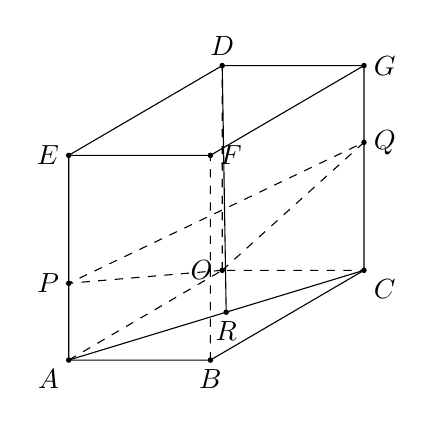
\begin{tikzpicture}[x={(-.65cm,-.38cm)},y={(.9cm,0cm)},z={(0cm,.65cm)}]
      \coordinate (O) at (0,0,0);\coordinate (A) at (3,0,0);
      \coordinate (B) at (3,2,0);\coordinate (C) at (0,2,0);
      \coordinate (D) at (0,0,4);\coordinate (E) at (3,0,4);
      \coordinate (F) at (3,2,4);\coordinate (G) at (0,2,4);
      \draw (A)--(B)--(C)--(G)--(F)--(E)--(A);
      \draw (E)--(D)--(G);\draw[dashed] (A)--(O)--(C) (O)--(D) (B)--(F);
      \coordinate (P) at (3,0,1.5);\coordinate (Q) at (0,2,2.5);\coordinate (R) at (1.4,1.0667,0);
      \draw[dashed] (O)--(P)--(Q)--cycle;\draw (A)--(C) (D)--(R);
      \foreach \p/\pos in {O/left,A/below left,B/below,C/below right,D/above,E/left,F/right,G/right,P/left,Q/right,R/below} {
        \fill (\p) circle (1pt) node[\pos] {$\p$};
      }
    \end{tikzpicture}
  \end{center}
  \caption{直方体と点$P,Q,R$の位置（模式図）}
\end{figure}
\begin{align}
  \overrightarrow{DR}=
  \begin{pmatrix}0\\2\\-4
  \end{pmatrix}
  +\alpha
  \begin{pmatrix}3\\-2\\0
  \end{pmatrix}
\end{align}
から
\begin{align}
  \overrightarrow{DR}\cdot\overrightarrow{OP}
  &=
  \begin{pmatrix}3\\0\\4s
  \end{pmatrix}\cdot
  \begin{pmatrix}3\alpha\\2-2\alpha\\-4
  \end{pmatrix}=0,\\
  \overrightarrow{DR}\cdot\overrightarrow{OQ}
  &=
  \begin{pmatrix}0\\2\\4t
  \end{pmatrix}\cdot
  \begin{pmatrix}3\alpha\\2-2\alpha\\-4
  \end{pmatrix}=0.
\end{align}
よって
\begin{align}9\alpha-16s=0,\qquad1-\alpha=4t.
\end{align}
だから$\alpha=\dfrac{16}{9}s=1-4t$であり，$0<s<1$，$0<t<1$から，この時常に$0<\alpha<1$となるので，
\begin{align}\dfrac{16}{9}s+4t=1.
\end{align}
\newpage

\section*{第2問}

% Source: handwritten.pdf 第2問．
% 原稿未収録: handwritten.pdf は5ページで，表紙，第1問，第3問，番号未記入の白紙，第5問からなる．
% 第2問に対応する解答ページが見当たらず，文字起こしは保留．解答の創作は行わない．
\newpage
\newpage

\section*{第3問}

% Source: handwritten.pdf 第3問．
{\bf [解]}
題意のようになるのは，$n$回目に$n$のカードを引くか，$n$の1つ上におかれているカードを引く時．

\subparagraph{(i) $n$回目に$n$のカードを引く時}
各回の試行で，引いたカードをより下の位置におくので，
\begin{align}\dfrac{1}{n}\cdot\dfrac{2}{n}\cdot\dfrac{3}{n}\cdots\dfrac{n-1}{n}.
\end{align}
さらに，$n$のカードは1番上に戻るので，
\begin{align}
  \dfrac{1}{n}\cdot\dfrac{2}{n}\cdots\dfrac{n-1}{n}\cdot\dfrac{1}{n}
  =\dfrac{(n-1)!}{n^n}.
\end{align}

\subparagraph{(ii) $n$回目に$n$の1つ上におかれたカードを引く時}
$1$〜$n-1$回目の試行のうち1回だけ，$n$の上にカードをおく．これを$k$回目の試行として，
\begin{align}
  \dfrac{1}{n}\cdot\dfrac{2}{n}\cdots\dfrac{k-1}{n}\cdot\dfrac{n-k}{n}
  \cdot\dfrac{k}{n}\cdots\dfrac{n-2}{n}.
\end{align}
さらに，$n$回目に引いたカードは$n$のカードの下におくので，
\begin{align}
  \dfrac{1}{n}\cdot\dfrac{2}{n}\cdots\dfrac{k-1}{n}\cdot\dfrac{n-k}{n}
  \cdot\dfrac{k}{n}\cdots\dfrac{n-2}{n}\cdot\dfrac{n-1}{n}
  =\dfrac{(n-1)!(n-k)}{n^n}.
\end{align}
$k$について足して
\begin{align}
  \dfrac{(n-1)!}{n^n}\sum_{k=1}^{n-1}(n-k)
  =\dfrac{(n-1)!}{n^n}\sum_{k=1}^{n-1}k
  =\dfrac{(n-1)!}{n^n}\cdot\dfrac{1}{2}n(n-1).
\end{align}
\casesend
以上から
\begin{align}
  \dfrac{(n-1)!\left\{1+\dfrac{1}{2}n^2-\dfrac{1}{2}n\right\}}{n^n}
  =\dfrac{(n-1)!(n^2-n+2)}{2n^n}.
\end{align}
\newpage

\section*{第4問}

% Source: handwritten.pdf 第4問．
% handwritten.pdf p.4 は「第 問」の問題番号が未記入で，本文も白紙．
% 第3問と第5問の間にあるので第4問の可能性があるが，番号は確認できない．
% 第4問として特定できる解答本文はなく，転記は保留（行列の問題）．
\newpage
\newpage

\section*{第5問}

% Source: handwritten.pdf 第5問．
{\bf [解]}
$c=\cos\theta$，$s=\sin\theta$とおく．$C$上の点$(X,Y)$とすると，
\begin{align}
  X=(2+c)c,\qquad Y=(2+c)s,\\
  X'=-2cs-2s=-2s(c+1),\\
  Y'=2c+\cos2\theta=2c^2+2c-1.
\end{align}
$0\leqq\theta\leqq\pi$で$X'\leqq0$かつ$Y\geqq0$だから，
$\theta=0$で$P(3,0)$，$\theta=\pi$で$P'(-1,0)$に達して，求める体積$V$として
\begin{align}
  \begin{split}
    V&=\int_{-1}^3\pi Y^2\,dX\\
    &=\int_{\pi}^0\pi\{(2+c)s\}^2\dfrac{dX}{d\theta}\,d\theta\\
    &=\pi\int_0^\pi(2+c)^2s^2\,2s(c+1)\,d\theta\\
    &=2\pi\int_0^\pi(2+c)^2(1-c^2)(c+1)s\,d\theta\\
    &=2\pi\int_0^\pi(-c^5-5c^4-7c^3+c^2+8c+4)s\,d\theta\\
    &=-2\pi\left[-\dfrac{1}{6}c^6-c^5-\dfrac{7}{4}c^4
    +\dfrac{1}{3}c^3+4c^2+4c\right]_0^\pi\\
    &=-2\pi\cdot2\left(1-\dfrac{1}{3}-4\right)\\
    &=\dfrac{40}{3}\pi.
  \end{split}
\end{align}
\newpage

\section*{第6問}

% Source: handwritten.pdf 第6問．
% 原稿未収録: handwritten.pdf は5ページで，最終ページは第5問の解答．
% 第6問に対応する解答ページが見当たらず，文字起こしは保留．解答の創作は行わない．
\newpage
\newpage

\end{document}
